\chapter{Construção de Protocolo de Experimentação}
\label{cp:construcao}

Neste capítulo é demonstrado o processo de construção de um protocolo de experimentação utilizando a ferramenta implementada neste trabalho, de modo a ilustrar o apoio que esta provê ao experimentador em cada fase do processo experimental, descrito pela Figura~\ref{ideia}. A apresentação é demonstrada de forma individual para cada fase: \textit{Definição}, \textit{Planejamento}, \textit{Operação}, \textit{Análise} e \textit{Empacotamento}.

Para a condução desta demonstração foi escolhido o experimento conduzido para avaliar a eficácia e a eficiência da Ferramenta de Visualização de Software \textit{SofVisOAH}~\cite{d2012avaliaccao}. Os dados que compõem o Pacote de Laboratório desse estudo foram utilizados para a instanciação do Pacote de Laboratório utilizando a ferramenta BPMN implementada neste trabalho.

\section{Experimento de Demonstração: Avaliação da \textit{SofVisOAH}}

O respectivo experimento de demonstração refere-se ao trabalho de ~\citeauthoronline{d2012avaliaccao}~(\citeyear{d2012avaliaccao}), que contextualiza como auxílio à área de Engenharia de Software, a Visualização de Software, a qual lida com a complexidade estrutural, apoiando tarefas de Compreensão de Programas por meio de representações visuais, permitindo interação com essas representações gráficas, provendo auxílio ao processo de entendimento. Uma ferramenta de Visualização de Software proporciona suporte ao usuário para obter informações por meio de análises dos artefatos visuais disponíveis, gerando assim, auxílio ao processo de entendimento de programas~\cite{d2012avaliaccao}.

O principal objetivo do experimento de ~\citeauthoronline{d2012avaliaccao}~(\citeyear{d2012avaliaccao}) é avaliar a utilização da ferramenta \textit{SofVisOAH} no apoio ao entendimento de Programas Orientados
a Aspectos, em detrimento ao entendimento de código convencional. Alguns fatores foram avaliados no experimento: verificação se a ferramenta auxilia na localização de defeitos assim como a compreensão de um Programa Orientado a Aspectos~\cite{d2012avaliaccao}.

Com a condução do experimento, os participantes puderam fornecer como respostas, além das medições que permitiram derivar métricas quantitativas relativas ao uso da ferramenta, uma avaliação qualitativa da mesma. Após a condução do experimento e avaliação dos resultados, foi possível constatar estatisticamente que a \textit{SofVisOAH} proveu auxílio às tarefas de Localização de Defeitos e Compreensão de Programa~\cite{d2012avaliaccao}.

\section{Elaboração do Protocolo de Experimentação}

\subsection{Fase de Definição}
Inicialmente devem ser definida uma visão geral relativa experimentação através dos itens estão descritos a seguir~\cite{d2012avaliaccao}:

\begin{itemize}

\item Objeto de Estudo -- Ferramenta de Visualização de Software \textit{SofVisOAH}.

\item Propósito -- avaliar e comparar a utilização da ferramenta \textit{SofVisOAH} como apoio a tarefas de Revisão de Programa em relação à Revisão de Programa Ad Hoc.

\item Enfoque de Qualidade -- Tempo, Quantidade de defeitos localizados e Entendimento do programa.

\item Perspectiva -- Do experimentador.

\item Contexto -- Laboratório de informática da Universidade Estadual Paulista Júlio de Mesquita Filho, Unesp, no campus da Faculdade de Ciências e Tecnologia.

\end{itemize}

A elaboração do modelo de processo de negócio, representado na Figura~\ref{img:protocolo-definicao}, explicita a sequência de atividades (Definir Objeto de Estudo, Definir Propósito, Definir Métrica, Definir Perspectiva e Definir Contexto) que devem ser executadas para a definição dos itens descritos acima, e seus respectivos artefatos produzidos. Todas as atividades executadas neste processo foram realizadas pelo Experimentador.

%figura DEFINICAO
\begin{figure}[!htb]
\centering
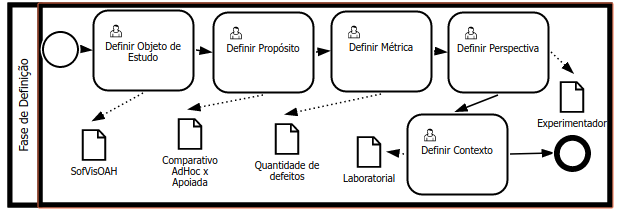
\includegraphics[width=0.85\textwidth]{images/protocolo-definicao.png}
\caption{Protocolo de Experimentação referente à Fase de Definição.}
\label{img:protocolo-definicao}
\end{figure}

A construção do processo referido na Figura~\ref{img:protocolo-definicao}, a partir da adição da piscina referente a Fase de Definição, é inserido o evento de início juntamente com as atividades listadas anteriormente, como cada atividade será executada pelo experimentador, essas devem ser da categoria \textit{User Task}. Por fim, a partir de cada atividade foram produzidos \textit{Data Objects} referentes as definições estabelecidas.

\subsection{Fase de Planejamento}
Na fase seguinte, devem ser definidos um conjunto de elementos de forma específica, dentre os quais: conjunto de questões e métricas (Figura~\ref{img:questoes}). Também foram planejadas hipóteses nulas e alternativas, ilustradas na Figura~\ref{img:hipoteses}, assim como, variáveis independentes (Figura~\ref{img:independentes}) e variáveis dependentes (Figura~\ref{img:dependentes})~\cite{d2012avaliaccao}.

%figura questoes
\begin{figure}[!htb]
\centering
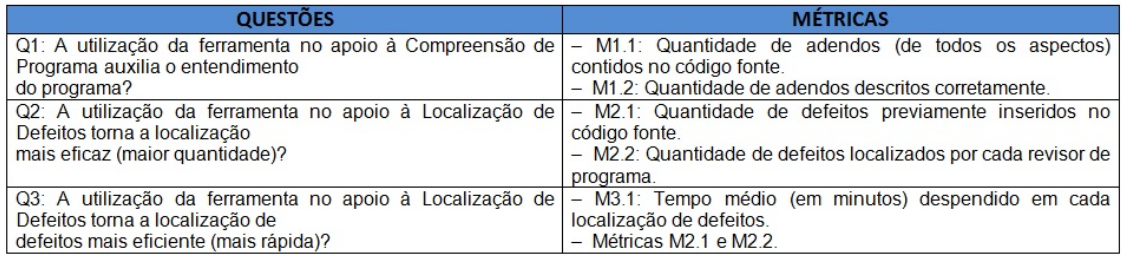
\includegraphics[width=0.9\textwidth]{images/tabela-questoes.png}
\caption{Questões e Métricas elaboradas na Atividade Planejamento~\cite{d2012avaliaccao}.}
\label{img:questoes}
\end{figure}

%figura hipotese
\begin{figure}[!htb]
\centering
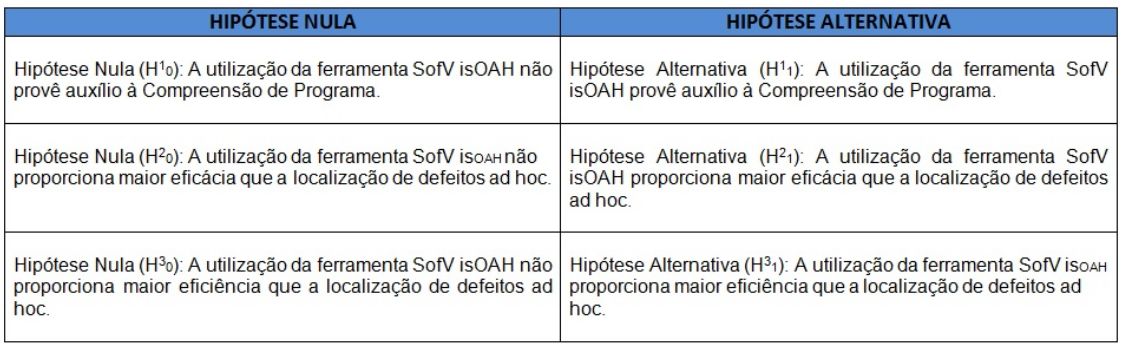
\includegraphics[width=0.9\textwidth]{images/tabela-hipoteses.png}
\caption{Hipóteses elaboradas na Atividade Planejamento~\cite{d2012avaliaccao}.}
\label{img:hipoteses}
\end{figure}

%figura independentes
\begin{figure}[!htb]
\centering
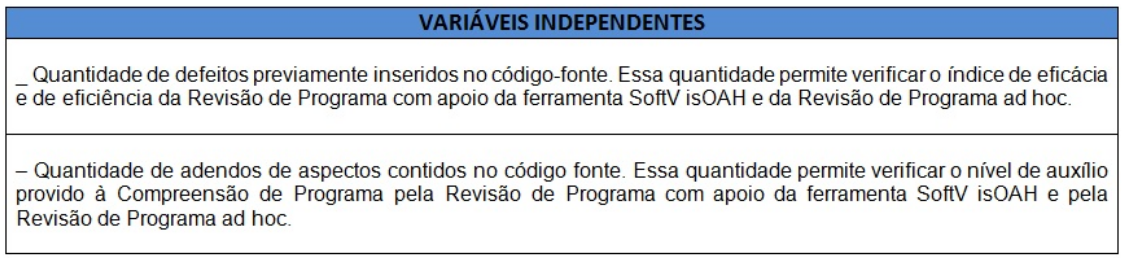
\includegraphics[width=0.9\textwidth]{images/tabelas-variaveis-independentes.png}
\caption{Variáveis Independentes elaboradas na Atividade Planejamento~\cite{d2012avaliaccao}.}
\label{img:independentes}
\end{figure}


%figura dependentes
\begin{figure}[!htb]
\centering
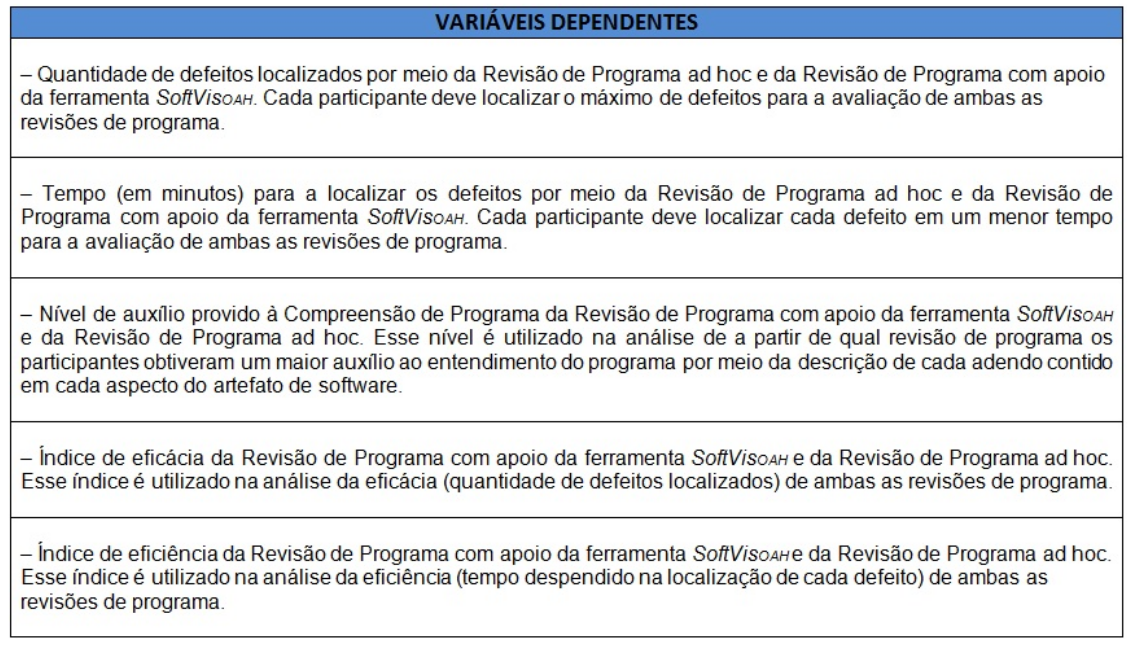
\includegraphics[width=0.9\textwidth]{images/tabelas-variaveis-dependentes.png}
\caption{Variáveis Dependentes elaboradas na Atividade Planejamento~\cite{d2012avaliaccao}.}
\label{img:dependentes}
\end{figure}


Em seguida, a Seleção de Participantes, os quais são escolhidos mediante seleção determinística, envolvendo alunos de graduação em Ciência da Computação~\cite{d2012avaliaccao}.

Por fim, foi definida a instrumentação, categorizada em dois tipos: Tecnologia e Artefato. Os instrumentos de Tecnologia foram definidos de acordo com os requisitos tecnológicos para a execução de ambas as revisões de programa e conhecimento prévio para a realização das mesmas. A instrumentação é dividida nos seguintes grupos: Ferramentas Informatizadas (Figura ~\ref{img:instrumentacao1}), Materiais de Realização de Testes (Figura~\ref{img:instrumentacao2}), Materiais de Treinamento (Figura~\ref{img:instrumentacao3}), Questionários (Figura~\ref{img:instrumentacao4}) e Formulários (Figura~\ref{img:instrumentacao5})~\cite{d2012avaliaccao}.

%figura
\begin{figure}[!htb]
\centering
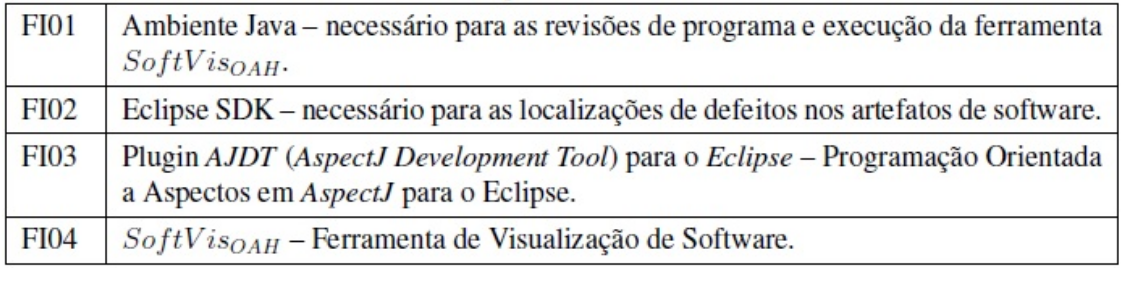
\includegraphics[width=0.9\textwidth]{images/tabela-instrumentacao1.png}
\caption{Instrumentação – Ferramentas Informatizadas – Planejamento~\cite{d2012avaliaccao}.}
\label{img:instrumentacao1}
\end{figure}

%figura
\begin{figure}[!htb]
\centering
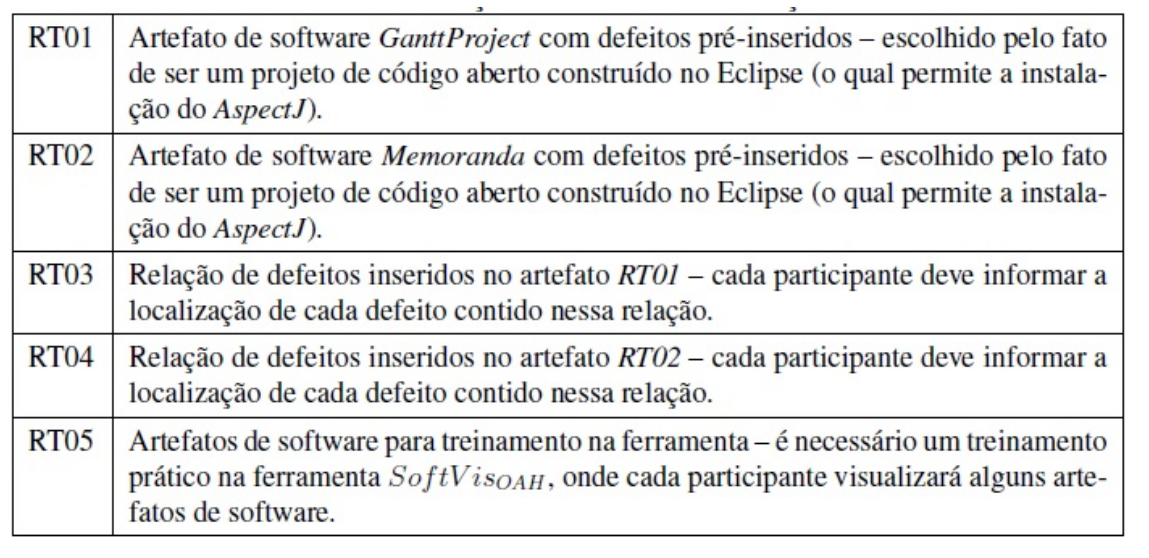
\includegraphics[width=0.9\textwidth]{images/tabela-instrumentacao2.png}
\caption{Instrumentação – Materiais de Realizacao de Testes – Planejamento~\cite{d2012avaliaccao}.}
\label{img:instrumentacao2}
\end{figure}

%figura
\begin{figure}[!htb]
\centering
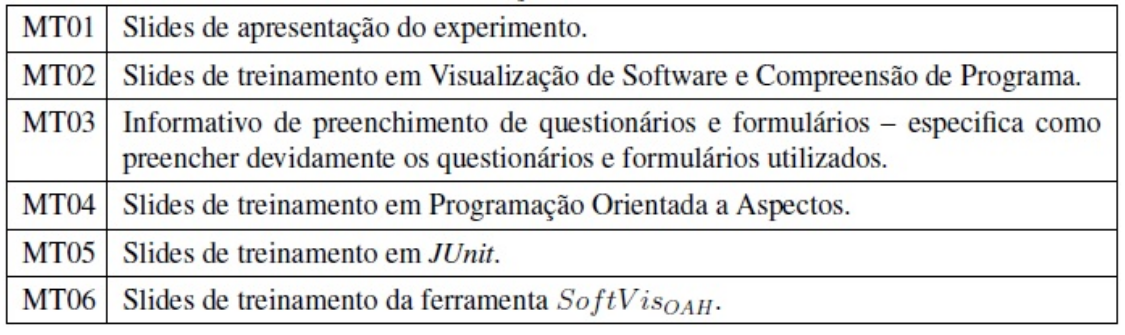
\includegraphics[width=0.9\textwidth]{images/tabela-instrumentacao3.png}
\caption{Instrumentação – Materiais de Treinamento – Planejamento~\cite{d2012avaliaccao}.}
\label{img:instrumentacao3}
\end{figure}

%figura
\begin{figure}[!htb]
\centering
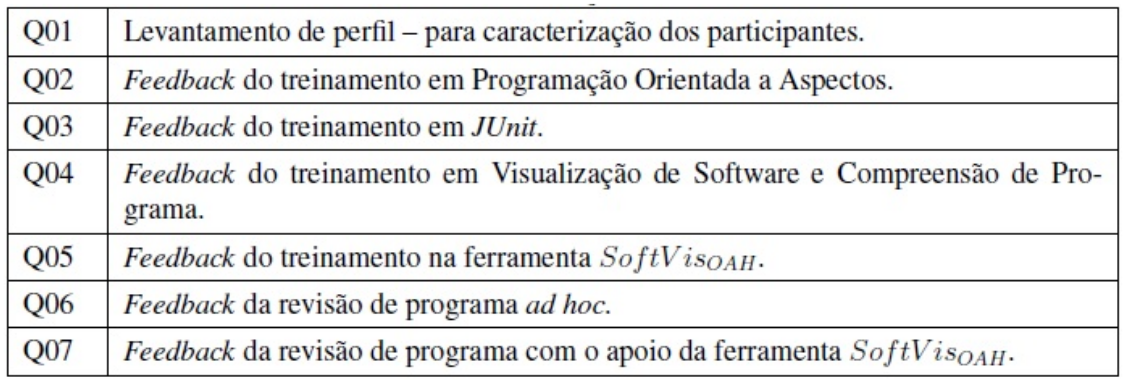
\includegraphics[width=0.9\textwidth]{images/tabela-instrumentacao4.png}
\caption{Instrumentação – Questionários – Planejamento~\cite{d2012avaliaccao}.}
\label{img:instrumentacao4}
\end{figure}

%figura
\begin{figure}[!htb]
\centering
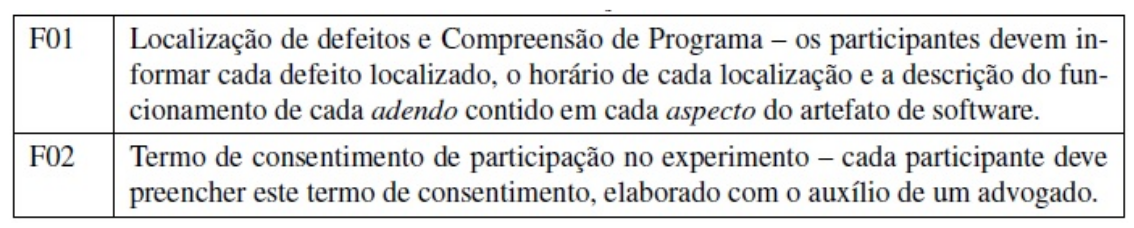
\includegraphics[width=0.9\textwidth]{images/tabela-instrumentacao5.png}
\caption{Instrumentação – Formulários – Planejamento~\cite{d2012avaliaccao}.}
\label{img:instrumentacao5}
\end{figure}

%%%%%%%%%%%%
%%%%%%%%%%%%
%figura PLANEJAMENTO
\begin{figure}[!htb]
\centering
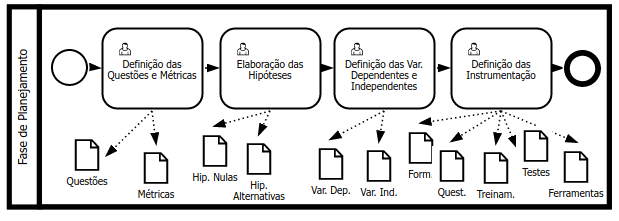
\includegraphics[width=0.85\textwidth]{images/protocolo-planejamento.png}
\caption{Protocolo de Experimentação referente à Fase de Planejamento.}
\label{img:protocolo-planejamento}
\end{figure}


O plano de execução da \textit{Fase de Planejamento}, representada pelo modelo de processo de negócio apresentado na Figura~\ref{img:protocolo-planejamento}, define as atividades a seguir: Definição das Questões e Métricas (visa a elaborar o que será avaliado e como será medido), Elaboração das Hipóteses (objetiva definir a efetividade da ferramenta sob as suposições), Definição das Variáveis Dependentes e Independentes (define quais fatores podem influenciar de forma direta e indireta e como estes serão tratados), e por fim, Definição da Instrumentação (define os instrumentos que serão utilizados no experimento como ferramentas de software, apresentações visuais, questionários e formulários). Todas as atividades desta fase são executadas pelo Experimentador.

A construção do diagrama referente a esta fase, representado na Figura~\ref{img:protocolo-planejamento}, inicia-se a partir da inserção da piscina referente a Fase de Planejamento e do evento de início. Em seguida, são adicionadas as atividades do tipo \textit{User Task}, pois todas atividades desta fase são referentes ao usuário, e por fim o evento de término. A partir destas atividades foram produzidos \textit{Data Objects} referentes às questões e métricas, hipóteses nulas e alternativas, variáveis dependentes e independentes e diversos artefatos, tais como formulários, questões, treinamentos, testes e ferramentas.

\subsection{Fase de Operação}
Para a execução deste experimento, o conjunto de participantes foi aleatoriamente dividido em dois grupos: os participantes de código ímpar foram alocados para o Grupo A e os demais para o Grupo B. Cada participante teve seu perfil caracterizado por meio de um questionário de levantamento de perfil através da \textit{OntoExpTool}. Os participantes realizaram os mesmos tipos de atividade, revisões de programa Ad Hoc e com o apoio da ferramenta \textit{SofVisOAH}, exercendo entendimento do programa e a localização de defeitos no código fonte~\cite{d2012avaliaccao}.

%%%%%%%%%%%%
%%%%%%%%%%%%
%figura OPERACAO
\begin{figure}[!htb]
\centering
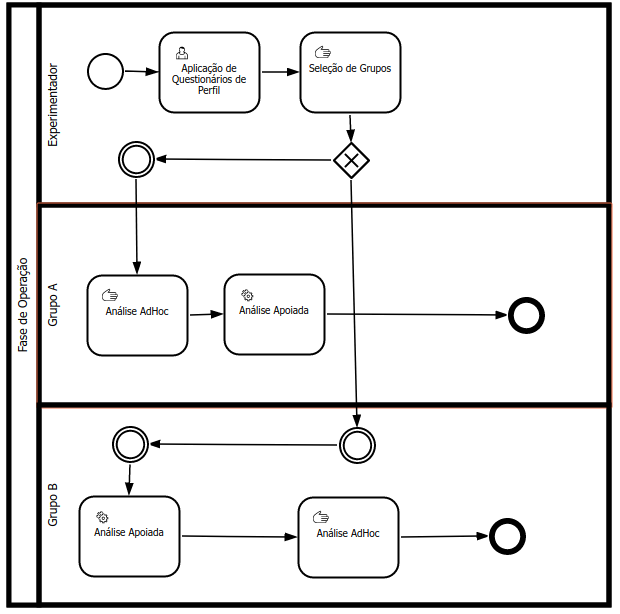
\includegraphics[width=0.85\textwidth]{images/protocolo-operacao.png}
\caption{Protocolo de Experimentação referente à Fase de Operação.}
\label{img:protocolo-operacao}
\end{figure}

Para esta fase, o modelo de processo respectivo, apresentado na Figura~\ref{img:protocolo-operacao}, define a execução de três processos relacionados. O primeiro, sob responsabilidade do Experimentador é composta pelas atividades: Aplicação de Questionários de Perfil (para todos os participantes são aplicadas questões sobre perfil, assim como do treinamento e revisão do programa) e Seleção de Grupos (separação dos participantes entre os dois grupos definidos). A partir da finalização do processo anterior, são iniciados os processos referentes aos participantes do Grupo A e B de forma concomitante, contendo as seguintes tarefas de forma alternada: Análise AdHoc (realiza-se o processo de detecção de defeitos sem qualquer auxílio automatizado) e Análise Apoiada (realiza-se a detecção de defeitos com o auxílio das técnicas de visualização apresentadas na ferramenta \textit{SofVisOAH}).

Em relação a construção do protocolo apresentado na Figura~\ref{img:protocolo-operacao}, inicialmente adiciona-se a piscina referente à Fase Operação, em seguida esta é dividida em três partes, uma cada categoria de atores. A execução inicia-se por meio da aplicação do questionário e seleção de grupos realizada pelo experimentador, logo, são adicionadas atividades para cada tarefa na parte referente ao experimentador. Após, são adicionadas as atividades de análise apoiada e Ad Hoc para cada grupo de modo alternado. Por fim, são adicionados os eventos de término.


\subsection{Fase de Análise e Interpretação}

Na análise executada no experimento, os participantes descreveram corretamente mais adendos de aspectos utilizando a \textit{SofVisOAH}. Em relação ao quesito auxílio à Compreensão de Programa, foi aplicado o Teste-T Bicaudal com Variação Desigual. Portanto, constata-se que a utilização da ferramenta provê auxílio à Compreensão de Programa~\cite{d2012avaliaccao}.

%%%%%%%%%%%%
%%%%%%%%%%%%
%figura ANALISE
\begin{figure}[!htb]
\centering
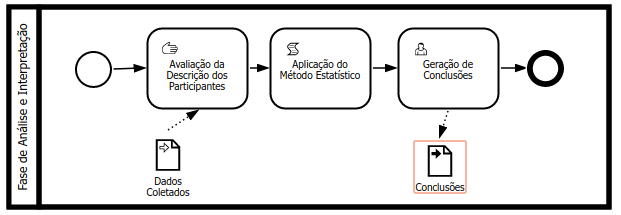
\includegraphics[width=0.85\textwidth]{images/protocolo-analise.png}
\caption{Protocolo de Experimentação referente à Fase de Análise e Interpretação.}
\label{img:protocolo-analise}
\end{figure}

Desse modo, a elaboração do modelo de processo, ilustrado na Figura~\ref{img:protocolo-analise} é composta pelas seguintes atividades, todas estas executadas pelo Experimentador: Avaliação da Descrição dos Participantes (foi realizada a extração dos dados coletados a partir de questionários e formulários sobre o perfil do participante e a ferramenta \textit{SofVisOAH}), Aplicação do Método Estatístico (a partir do conjunto de dados foi aplicado o Teste-T) e Geração de Conclusões (através da finalização do teste estatístico juntamente com as hipóteses e variáveis definidas foi estabelecido o conjunto de conclusões sobre o objeto em investigação).

Para esta fase, a elaboração do protocolo de experimentação (Figura~\ref{img:protocolo-analise}), inicia-se com a adição do piscina e do início de evento e seguido das respectivas atividades indicadas. Como entrada do processo, indicado pelo \textit{Data Input} têm-se os dados coletados na fase anterior, os quais são vinculados com a primeira atividade. Como resultado da terceira atividade foram obtidas as conclusões do estudo, indicadas por meio de um \textit{Data Output}. De modo a encerrar, adiciona-se o evento de término.


\subsection{Fase de Empacotamento e Apresentação}

Como último passo, a \textit{Fase de Empacotamento e Apresentação}, os dados de todo o transcorrer do experimento foram armazenados em uma base de dados e após da fase anterior, o Pacote de Laboratório deste experimento foi instanciado em dois formatos: XML e OWL, permitindo ser visualizados na própria ferramenta~\cite{d2012avaliaccao}.

Também foi criado um pacote compactado contendo o	s arquivos descritos acima, e todos os artefatos e documentos provenientes do estudo, desse modo, disponíveis para análises e futuras replicações~\cite{d2012avaliaccao}. 

%%%%%%%%%%%%
%%%%%%%%%%%%
%figura EMPACOTAMENTO
\begin{figure}[!htb]
\centering
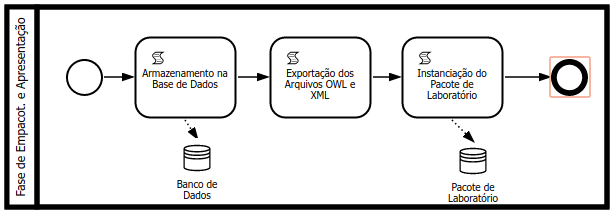
\includegraphics[width=0.85\textwidth]{images/protocolo-empacotamento.png}
\caption{Protocolo de Experimentação referente à Fase de Empacotamento e Apresentação.}
\label{img:protocolo-empacotamento}
\end{figure}

Por fim, o modelo de processo de negócio (ilustrado na Figura~\ref{img:protocolo-empacotamento}) representa o protocolo de execução da \textit{Fase de Empacotamento e Apresentação}, que neste experimento é composta pela seguintes atividades: Armazenamento na Base de Dados (são obtidos todos os conjuntos de dados gerados nas atividades das fases anteriores), Exportação dos Arquivos OWL e XML (processamento e geração destes arquivos) e, Instanciação do Pacote de Laboratório (encapsulamento dos dados relativos ao experimento juntamente com todos seus artefatos), todas atividades executadas pelo Experimentador.

O plano de execução referente a essa etapa, inicia-se a partir da adição da piscina dessa fase e o início de evento. Em seguida, foram adicionadas atividades automatizadas (\textit{Script Task}), para o armazenamento dos dados em um Banco de Dados e na forma de Pacote de Laboratório, ambos representados por \textit{Data Store}. Concluindo, é adicionado o evento de término.

\section{Considerações Finais}
Neste capítulo foi apresentado o processo de concepção do protocolo de experimentação (plano de execução) em experimentos controlados. A partir da realização das atividades em cada fase, novos componentes são atrelados ao corpo de experimento, em que a partir de versões iniciais são refinados nas fases subsequentes, por exemplo, o conjunto de hipóteses que foi definido e aprimorado nas fases de Definição e Planejamento, respectivamente, também está presente na fase de Análise e Interpretação atuando como uma entrada de dados para esta fase.
Além disso, é possível perceber as relações e dependências entre atividades de diferentes fases do estudo experimental.